%234567890          1234567890          1234567890          1234567890
%         1234567890          1234567890          1234567890          1234567890
\documentclass[a4paper,11pt,twoside]{report}
\usepackage{dotss}
\usepackage{xr}
\usepackage{a4wide}
\usepackage{amsmath}
\usepackage{amssymb}

\begin{document}
\newcommand{\coursename}{Visualization (2IV35)}
\newcommand{\doctitle}{Practical assignment }
\newcommand{\docversion}{0.1}
\newcommand{\docdate}{\today}

\newcommand{\imagescalefactor}{0.40}
\newcommand{\cref}[1]{chapter \ref{#1}}

% \dotsspreamble

% \tableofcontents

\dotssdocument

% \chapter{Introduction}
% 	This report contains the documentation of the process of developing an visualisation tool for the practical assignment of the course 2IV35 - Visualization. The goal of the practical assignment was to develop a progam in a language of choice to visualize a given flow-simulation. The development of this progam took an incremental approach, adding new features to the progam over the course of several weeks as new topics had been discussed during the lectures. Key to the success of the visualisation was that is should remain `interactive', e.g. the user should be able to see the results of actions on his or her part visualized in real-time.
%
% 	In the next chapter (\cref{overview}) we give a general description of the progam that we have developed, and in \cref{detaileddescription} we give a detailed description of every step in the development process.

% \chapter{Overview}\label{overview}
% 	In this chapter we give a short, general overview of the design proces of the progam and of the progam itself.
%
% 	The development of the progam was guided by the overview as given on the course website. This meant that on average every two weeks a new part of the progam should be completed. The first 3 steps were completed relatively quickly (although there were some obstacles) leaving most of the time for the `main course' of steps 4-7. We chose to take the left branch (as depicted in \ref{fig:step1}) of the assignment, which meant we had to implement a way to visualize the divergence of a vector-field, isosurfaces over a scalar field, heightplotting and stream tubes. The choice was made quite early on before we had a clear understanding of the later steps, and can thus be considered arbitrary.
%
% 	We decided to build the program using the Java language. This decision was mode for a number of reasons. First of all an example program in Java was provided, providing a base for further development. Although an implementation in C was also available; we prefered Java because we were already more familiar with Java than C. As an added bonus Java provides cross-platform usability with a minimum of effort. This meant that we could develop the program under each member's prefered operating system. Furthermore it was noticed that the provided source code was compatible with the Java 1.4 specification which allowed use of the `Jikes' compiler. The reason to prefer Jikes over the Java compiler provided by Sun is that it is a very fast compiler (an order of magnitude faster) with little to no runtime penalty. We thus opted to not make use of some of the features offered by newer versions of the Java language to enable the use of the faster Jikes compiler. This combined means that the program runs under Windows as wel as Linux (and possibly, although untested, other Unix-like) based operating systems.
%
% 	As for the design of the progam itself an iterative approach was combined with extreme-progamming. This meant we only planned ahead for `big' features, and often refining completed steps into a more generic form for later steps. A good example of this is the side-panel which provides the main interface to the program. At first this consisted of little more than a few controls, but as soon as we came to the second step we realized that a lot of the following assignments required similar options. Therefore we opted to construc a generic base-panel which provides options such as the choice of dataset, scaling and clamping options and controls for constructing gradients. This base panel was then used to provide an interface for each of the main steps' controls.
%
% 	\begin{figure}[h]
% 	\centering
% 	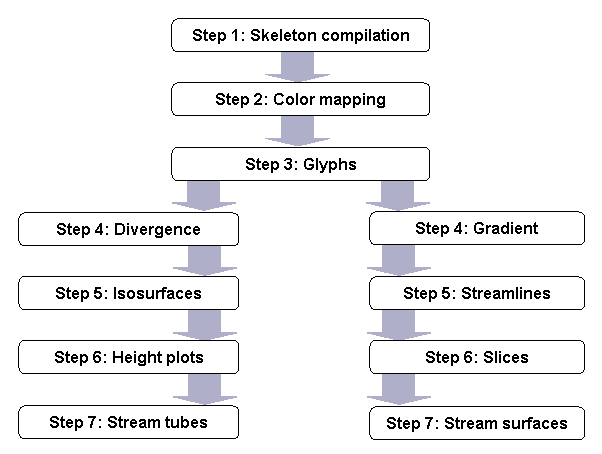
\includegraphics[scale=\imagescalefactor]{images/overview.png}
% 	\caption{The suggested workflow.}\label{fig:overview}
% 	\end{figure}

\chapter{Detailed description}\label{detaileddescription}
% 	\section{Skeleton compilation}
% 		This step does not really warrant much discussion. The only reasons to include it in our discussion here is to show what the progam looked like when we first used it, and to point out one problem that we encountered at this point. The problems lies in an (in our opinion) flaw in the given source code, which uses an GLJPanel. The problem is that a GLJPanel is very slow, giving low framerates under Windows, and unacceptable framerates  under Linux. The solution we used was to simply replace the GLJPanel with a GLCanvas which is much faster. One problem with this approach was pointed out by dr.ir. H. van de Wetering which is that when embedding a GLCanvas in other Swing controls there may be some problems with the drawing of the visualisation. However since we placed the Swing gui-elements next to the visualisation windows we did not have any problems.
% 		\begin{figure}[h]
% 		\centering
% 		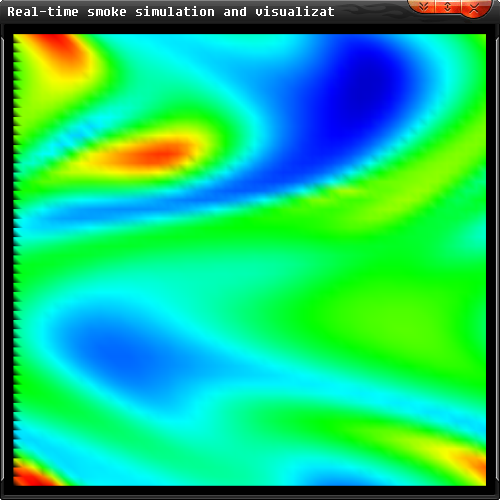
\includegraphics[scale=\imagescalefactor]{images/step1.png}
% 		\caption{The initial look of the progam.}\label{fig:step1}
% 		\end{figure}
% 		\newpage
% 	\section{Color mapping}
% 		The first real task was to set up a mechanism to implement color mapping. We choose to first do this as straight forward as possible and put all controls for the program on the same panel. In later versions of the progam some of these controls would be put on a tab of their own. The dataset selection, scaling and clamping and colormapping boxes would later be factored into a reuseable component.
%
% 		We have provided controls to select the dataset to visualize. Possible choices are density (rho or $\rho$) which indicates the density of the fluid simulation, force ($|$f$|$ or $|\overrightarrow{F}|$) which indicates the \emph{ammount} of force being applied at a certain point and velocity ($|$v$|$ or $\overrightarrow{v}$) which indicates the \emph{ammount} of movement of the fluid.
%
% 		It is also possibly to enable `scaling' and `clamping'. What scaling does is to scale sample-values that are read from the simulation to the range $[0..1]$. This is done by keeping track of the highest and lowest recorded sample-values in the previous frame, and using this to scale values read for the current frame. This makes the flow easier to see as the entire scale of the color-map will always be used, e.g. the highest peak will correspend to the high-end of the color-map and the lowest valley will correspend to the low-end of the color-map regardless of the actual values of those peaks and valleys.
% 		Clamping simply clamps the sample-values are read from the simulation to a user specifiably range. This means that the lowest possible value that can be read from the simulation is equal to the user-set lower bound, and similarly so for the highest possible value.
% 		Note that clamping is applied before scaling, allowing for the option to use the entire range of the color-map to visualize just a part of the sample-values generated by the simulation.
%
% 		Furthermore it is possible to specify a color-map to apply to the simulation. Three pre-defined colormaps are available, as well as one user definable colormap. The available predefined color-maps are a `rainbow' colormap which unsurprisingly consists of all colors present in a rainbow, a grayscale map where higher values are colored brighter, and a `Defined' map which is essentially the `rainbow' colormap with a limited number of gradient steps. For all of these color-maps it is possible to specify the number of steps in which the gradient should be divided by using a slider.
% 		A user can design his or her own favorite colormap by using the `Custom' setting. Colors can be added, changed or removed by right-clicking on a color and selecting the appropriate option. A minimum of at least two colors must be present, but no restriction is placed on the uniqueness of colors. Thus any gradient (even a single color) can be designed easily.
%
% 		One interesting feature that we added after seeing it in action on another groups visualisation is the use of texture mapping for the application of the color-map to the simulation grid. To this end we construct a one-dimensional texture which holds the gradient that the user has selected and use the sample-values at the grid points as in texture coordinate into this texture. The advantage of this method over the use of simply specifying a color for each grid-point is best seen when the number of colors in the color-map is low. By specifying that the texture mapping algorithm should use `nearest-neighbour' interpolation over the polygon we obtain sharp edges along the color-bands, instead of the more blurred look that would otherwise be obtained. This better matches the definition of the color-map as is also visible in the preview window.
% 		\begin{figure}[h]
% 		\centering
% 		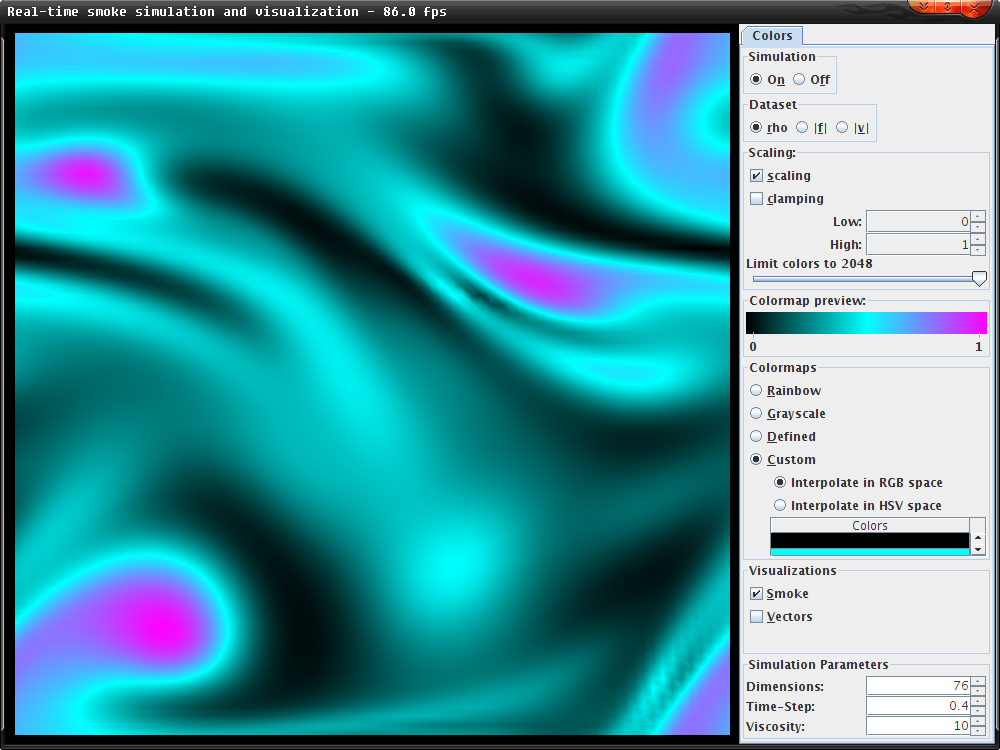
\includegraphics[scale=\imagescalefactor]{images/step2.png}
% 		\caption{The first gui elements.}\label{fig:step2}
% 		\end{figure}
% 		\newpage
	\section{Glyphs}
		\begin{figure}[h]
		\centering
		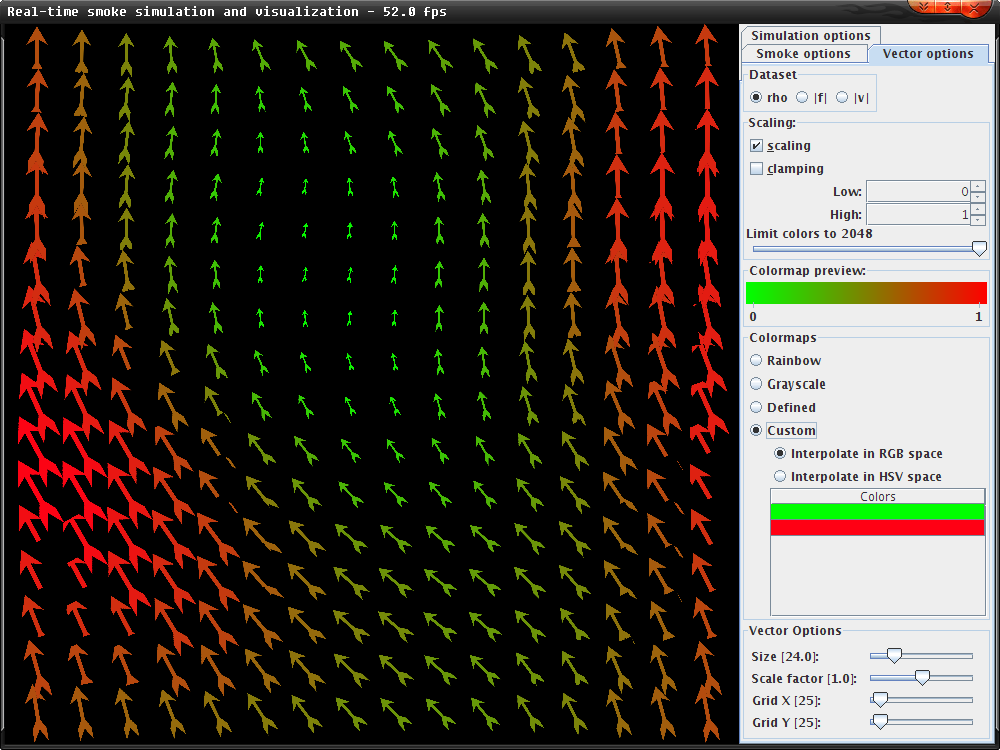
\includegraphics[scale=\imagescalefactor]{images/step3.png}
		\caption{Adding glyphs.}\label{fig:step3}
		\end{figure}
		\newpage
	\section{Divergence}
		\begin{figure}[h]
		\centering
		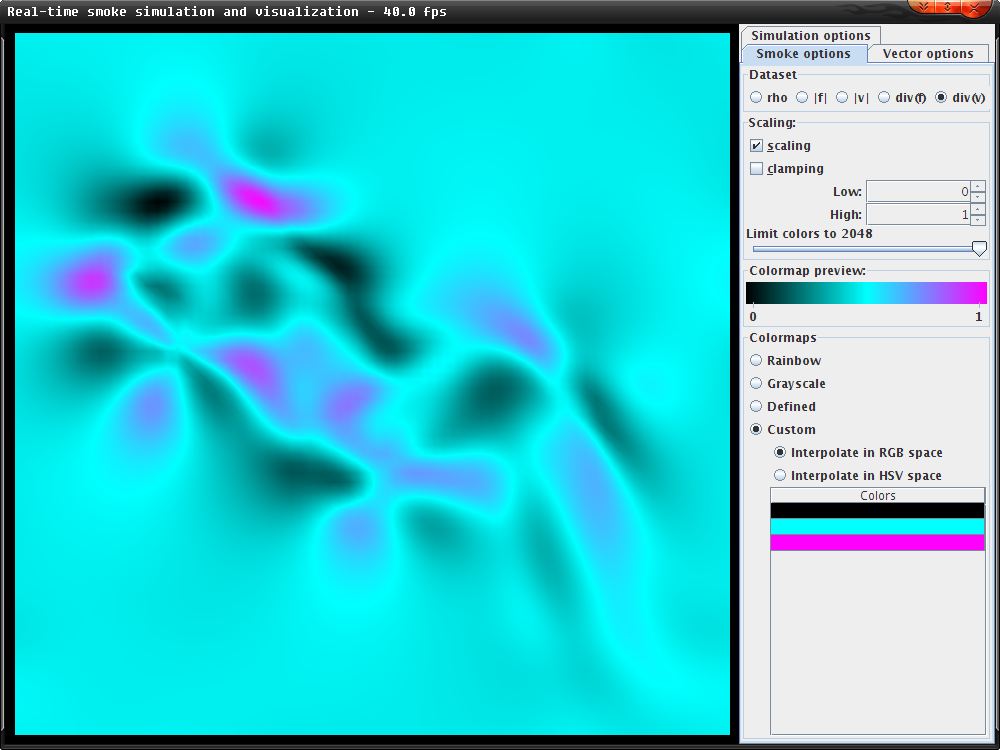
\includegraphics[scale=\imagescalefactor]{images/step4.png}
		\caption{Visualizing divergence.}\label{fig:step4}
		\end{figure}
		\newpage
	\section{Isosurfaces (Isolines)}
		\begin{figure}[h]
		\centering
		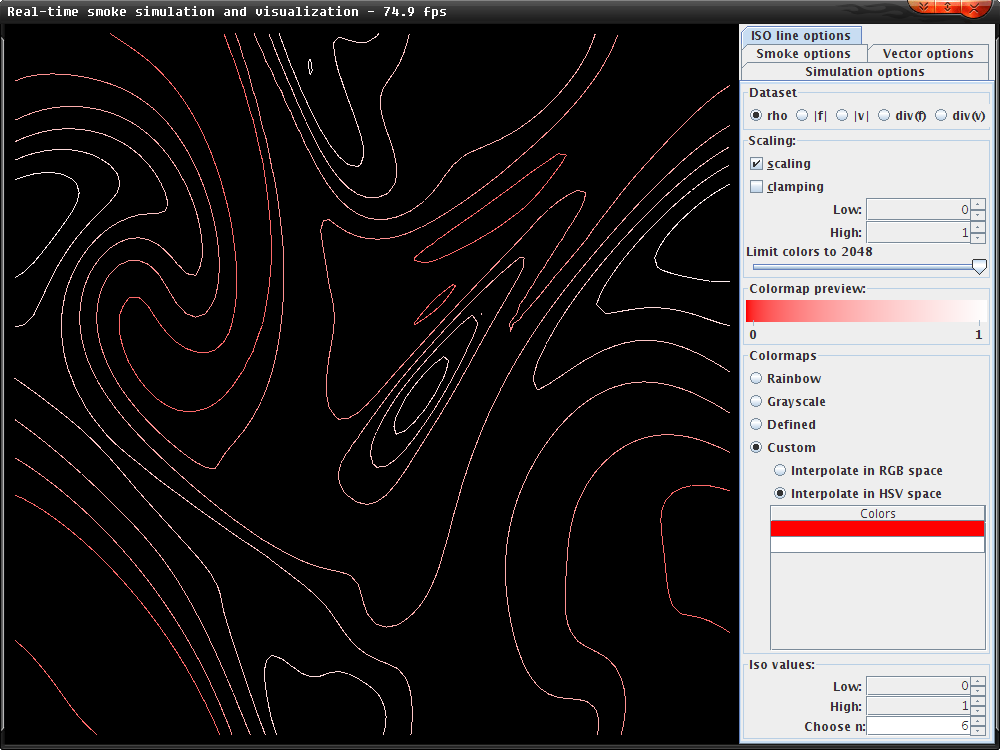
\includegraphics[scale=\imagescalefactor]{images/step5.png}
		\caption{Drawing isolines.}\label{fig:step5}
		\end{figure}
		\newpage
	\section{Height plots}
		\begin{figure}[h]
		\centering
		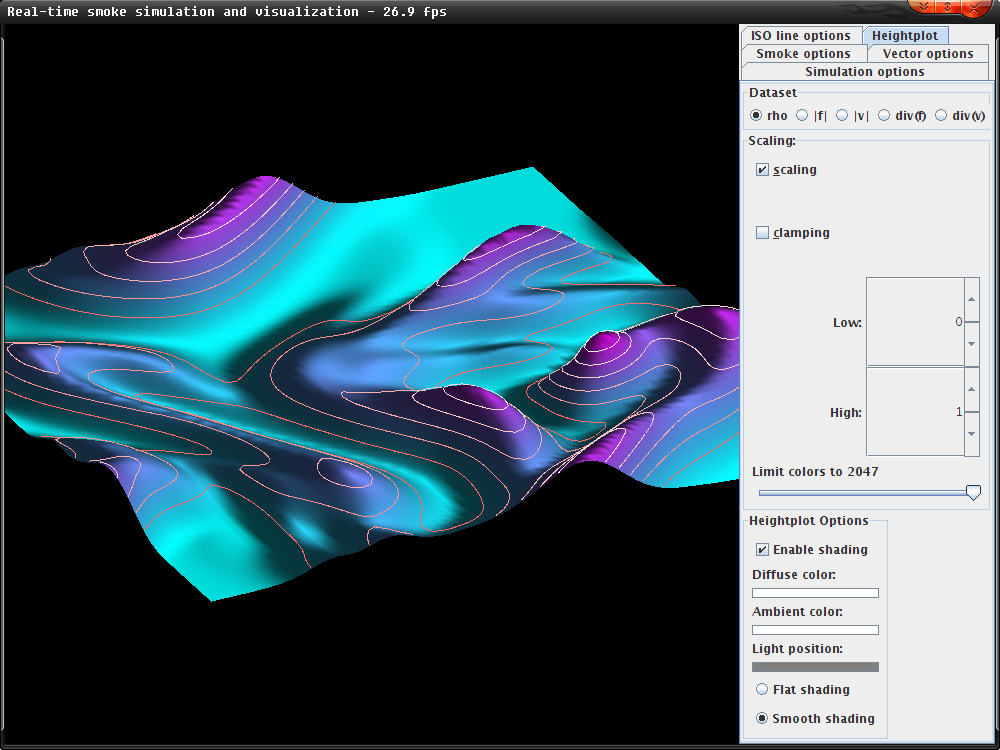
\includegraphics[scale=\imagescalefactor]{images/step6.png}
		\caption{The heightplot.}\label{fig:step6}
		\end{figure}
		\newpage
	\section{Stream tubes}
	% Oeps nog niet gecode...
\chapter{Conclusion}
% klein stukje slap gezever
\end{document}
